% Human-readable account of work/kkr-extremal: extremal equal-spin EGB black
% holes built directly at T = 0, reproduction of arXiv:2303.12471 and the
% extremal mass shift. Every number in the text is a macro from
% ../report/numbers.tex (generated by make_report_numbers.py from the data).
% Build:  pdflatex kkr-extremal-writeup.tex (twice)
% HTML:   python build_html.py   (same source, MathJax for the formulas)
\documentclass[11pt,a4paper]{article}
\usepackage[T1]{fontenc}
\usepackage{lmodern}
\usepackage[margin=2.5cm]{geometry}
\usepackage{amsmath,amssymb}
\usepackage{booktabs}
\usepackage{graphicx}
\usepackage{xcolor}
\usepackage[section]{placeins}
\usepackage[colorlinks=true,allcolors=blue!55!black]{hyperref}
% generated by make_report_numbers.py; do not edit
\newcommand{\Rgammamin}{1.773}
\newcommand{\Rgammaminy}{0.029}
\newcommand{\Rgammaymax}{36.3}
\newcommand{\Rgammacrosstwo}{0.71}
\newcommand{\Rgammacrossthree}{4.51}
\newcommand{\Rgammasmally}{0.0009}
\newcommand{\Rdigitworst}{3.7\times10^{-4}}
\newcommand{\Rconvaalpha}{0.05}
\newcommand{\Rconvamu}{2.3280174}
\newcommand{\Rconvamums}{2.3280172}
\newcommand{\Rconvay}{0.0568894}
\newcommand{\Rconvayms}{0.0568895}
\newcommand{\Rconvbalpha}{0.2}
\newcommand{\Rconvbmu}{2.5319363}
\newcommand{\Rconvbmums}{2.5319363}
\newcommand{\Rconvby}{0.2290601}
\newcommand{\Rconvbyms}{0.2290603}
\newcommand{\Rconvcalpha}{0.5}
\newcommand{\Rconvcmu}{2.8885348}
\newcommand{\Rconvcmums}{2.8885349}
\newcommand{\Rconvcy}{0.5112438}
\newcommand{\Rconvcyms}{0.5112439}
\newcommand{\Rbranchpoints}{268}
\newcommand{\Ralphamax}{3.118}
\newcommand{\Rymax}{2.443}
\newcommand{\Rxmax}{0.863}
\newcommand{\Rjlast}{0.189}
\newcommand{\Rnmaxbranch}{312}
\newcommand{\Rconstraintworst}{7.3\times10^{-5}}
\newcommand{\Rdmuworst}{7.4\times10^{-5}}
\newcommand{\Rdslopeworst}{8.7\times10^{-3}}
\newcommand{\Rcleanrows}{183}
\newcommand{\Rfirstlawworst}{3.7\times10^{-6}}
\newcommand{\Rfirstlawmedian}{7.2\times10^{-8}}
\newcommand{\Rsmarrworst}{2.8\times10^{-5}}
\newcommand{\Rsmarrmedian}{5.4\times10^{-7}}
\newcommand{\Romegaidclean}{5.2\times10^{-5}}
\newcommand{\Rvonedev}{3.3\times10^{-6}}
\newcommand{\RhHdev}{2.4\times10^{-7}}
\newcommand{\Rsigmanhdev}{3.8\times10^{-4}}
\newcommand{\Romegaiddev}{1.2\times10^{-2}}
\newcommand{\Rslopemin}{1.0710}
\newcommand{\Rslopeminy}{0.195}
\newcommand{\Rslopelast}{2.1775}
\newcommand{\Rmugrowth}{203}
\newcommand{\RkkraHdev}{6.5\times10^{-4}}
\newcommand{\RkkraHdevj}{1.2\times10^{-3}}
\newcommand{\Rkkrsdev}{1.4\times10^{-3}}
\newcommand{\Rkkrsdevj}{2.6\times10^{-3}}
\newcommand{\Rpolishedcouplings}{12}
\newcommand{\Rdmuworstms}{6.2\times10^{-6}}
\newcommand{\Rdpsiworstms}{1.9\times10^{-5}}
\newcommand{\Rdyworstms}{3.4\times10^{-7}}
\newcommand{\Rpsiratioworst}{1.8\times10^{-3}}
\newcommand{\Rcomparisontable}{%
  $0.005$ & $0.004790$ & $2.2115781$ & $9.9\times10^{-7}$ & $2.2115792$ & $1.3\times10^{-3}$ & $2.990940$ & $5.4\times10^{-6}$ & $2.990943$ & $1.1\times10^{-1}$ \\
  $0.01$ & $0.009845$ & $2.2262777$ & $7.1\times10^{-7}$ & $2.2262788$ & $7.7\times10^{-4}$ & $2.824561$ & $3.5\times10^{-6}$ & $2.824558$ & $8.8\times10^{-2}$ \\
  $0.02$ & $0.020720$ & $2.2550577$ & $1.2\times10^{-6}$ & $2.2550579$ & $1.6\times10^{-3}$ & $2.472846$ & $4.4\times10^{-6}$ & $2.472827$ & $1.6\times10^{-1}$ \\
  $0.035$ & $0.038427$ & $2.2944442$ & $9.4\times10^{-7}$ & $2.2944380$ & $8.4\times10^{-4}$ & $2.000655$ & $2.0\times10^{-6}$ & $2.000660$ & $9.0\times10^{-2}$ \\
  $0.05$ & $0.056889$ & $2.3280166$ & $8.0\times10^{-7}$ & $2.3280172$ & $5.7\times10^{-6}$ & $1.659079$ & $9.0\times10^{-7}$ & $1.659080$ & $8.6\times10^{-3}$ \\
  $0.075$ & $0.087750$ & $2.3734822$ & $2.2\times10^{-7}$ & $2.3734823$ & $9.1\times10^{-6}$ & $1.325970$ & $9.2\times10^{-8}$ & $1.325970$ & $2.4\times10^{-3}$ \\
  $0.1$ & $0.117873$ & $2.4107272$ & $1.5\times10^{-6}$ & $2.4107287$ & $3.7\times10^{-5}$ & $1.166215$ & $1.9\times10^{-8}$ & $1.166214$ & $8.3\times10^{-4}$ \\
  $0.15$ & $0.175201$ & $2.4739927$ & $4.7\times10^{-7}$ & $2.4739932$ & $1.1\times10^{-5}$ & $1.071493$ & $1.3\times10^{-7}$ & $1.071492$ & $2.3\times10^{-3}$ \\
  $0.2$ & $0.229060$ & $2.5319360$ & $4.3\times10^{-7}$ & $2.5319363$ & $8.8\times10^{-6}$ & $1.090071$ & $1.5\times10^{-7}$ & $1.090070$ & $2.8\times10^{-3}$ \\
  $0.3$ & $0.329212$ & $2.6465810$ & $1.2\times10^{-6}$ & $2.6465821$ & $4.5\times10^{-6}$ & $1.207815$ & $4.1\times10^{-7}$ & $1.207813$ & $2.1\times10^{-3}$ \\
  $0.4$ & $0.422511$ & $2.7651786$ & $1.2\times10^{-6}$ & $2.7651797$ & $4.6\times10^{-6}$ & $1.333843$ & $4.3\times10^{-7}$ & $1.333842$ & $2.7\times10^{-3}$ \\
  $0.5$ & $0.511244$ & $2.8885340$ & $8.0\times10^{-7}$ & $2.8885349$ & $1.1\times10^{-6}$ & $1.444398$ & $3.5\times10^{-7}$ & $1.444398$ & $6.2\times10^{-4}$ \\
}
\newcommand{\Rgcplateau}{38}

\newcommand{\ext}{\mathrm{ext}}

\title{Extremal rotating black holes in five-dimensional\\
Einstein--Gauss--Bonnet gravity, constructed directly at zero temperature}
\author{BHs project, \texttt{work/kkr-extremal}\\[2pt]
\small computation and write-up: Claude (Anthropic), working in this repository}
\date{7 October 2026}

\begin{document}
\maketitle

\begin{abstract}
We construct the extremal (zero-temperature) black holes of five-dimensional
Einstein--Gauss--Bonnet gravity that carry two equal angular momenta, directly
at $T=0$ and not as a limit of hot solutions. The construction follows the
radial gauge of Kleihaus, Kunz and Radu \cite{KKR2023}, in which the degenerate
horizon sits at the origin. We combine it with a spectral collocation method in
which the mass is read as a \emph{value} at infinity rather than as a derivative.
Two hidden zero modes of that gauge had to be identified and removed before the
problem became well posed. With these solutions we reproduce the extremal
boundary of the domain of existence in figure~1 of \cite{KKR2023}, to the
accuracy with which the published curves can be read. We then compute the
extremal mass $M_\ext(J,\alpha)$ and its slope
$\partial M_\ext/\partial\alpha|_J$ at fixed angular momentum, the slope
directly at $T=0$ by implicit differentiation of the discrete equations. These
agree with the zero-temperature extrapolation of non-extremal solutions in this
project's manuscript to a few parts in $10^{6}$. That is far better than the
uncertainty the manuscript attaches to its own slope. Along the way we find that
the extremal horizon is not smooth at finite coupling: a perturbation of the
near-horizon geometry grows with a non-integer power of the distance to the
horizon. This rules out an exact power-series description of the solutions at
the horizon.
\end{abstract}

\tableofcontents

\section{Introduction}

In Einstein gravity a rotating black hole cannot carry an arbitrary angular
momentum at a given mass. For the five-dimensional Myers--Perry solution with two
equal angular momenta $J_1=J_2=J$ the bound is
$M\ge\tfrac32\pi^{1/3}J^{2/3}$ (in units $G=1$). The black hole that saturates it
is \emph{extremal}: its Hawking temperature vanishes and its horizon becomes
degenerate. Adding a Gauss--Bonnet term to the action,
\begin{equation}
  I=\frac{1}{16\pi}\int d^5x\,\sqrt{-g}\,\bigl(R+\alpha L_{\rm GB}\bigr),\qquad
  L_{\rm GB}=R^2-4R_{\mu\nu}R^{\mu\nu}+R_{\mu\nu\rho\sigma}R^{\mu\nu\rho\sigma},
  \label{eq:action}
\end{equation}
moves that bound. The question this project's manuscript asks is how far, and in
which direction, once $\alpha$ is no longer small. To first order the answer is
known \cite{MaLiLu2020}:
\begin{equation}
  M_\ext=\tfrac32\pi^{1/3}J^{2/3}+\pi\alpha+\mathcal O(\alpha^2).
  \label{eq:firstorder}
\end{equation}

There are two ways to reach the extremal solutions at finite coupling. The
manuscript follows non-extremal black holes towards low temperature at fixed
$\alpha$ and extrapolates to $T=0$. It obtains the slope
$\partial M_\ext/\partial\alpha|_J$ as the zero-temperature limit of a
thermodynamic potential $\Psi$ conjugate to $\alpha$. Kleihaus, Kunz and Radu
(KKR below) \cite{KKR2023} instead built the extremal black holes
\emph{directly}, in a radial gauge that puts the degenerate horizon at $r=0$.
They used them to map the domain of existence of the family. They published
curves in figure~1 of their paper, but no tables, no stated accuracy and no
mass curve $M_\ext(J,\alpha)$.

The aim of the work reported here was therefore threefold:
\begin{enumerate}
\item rebuild KKR's direct construction and check it against their published
curves;
\item use it to obtain $M_\ext(J,\alpha)$ and its slope at $T=0$ \emph{without
any extrapolation in temperature}, and so test the manuscript's extrapolated
numbers by an independent route;
\item understand why the direct construction is numerically hard. It took
several failed attempts, and the reasons turned out to be physical.
\end{enumerate}

The main results are the following. The extremal solutions were constructed for
$0\le\alpha\le\Ralphamax$ in units of the horizon size, which covers
$0\le x\le\Rxmax$ in KKR's variable $x=3\pi\alpha/4M$. KKR's extremal curves are
reproduced to about $10^{-3}$, the precision to which their figure can be read.
At the manuscript's twelve couplings the extremal mass agrees with the
manuscript's extrapolation to $\Rdmuworstms$ and the slope to $\Rdpsiworstms$.
The slope starts at the perturbative value $\pi$, falls to $\Rslopemin$ and rises
again. And the extremal horizon is only $C^1$ in the natural radial coordinate,
because of a near-horizon mode with a non-integer exponent.

The rest of the report is organised as follows. Section~\ref{sec:model} sets up
the metric, the conserved quantities and the reduced variables.
Section~\ref{sec:nh} studies the near-horizon geometry and finds the non-smooth
mode. Section~\ref{sec:method} describes the numerical method, including the
attempts that failed and why. Section~\ref{sec:checks} lists the checks.
Section~\ref{sec:results} presents the results, and section~\ref{sec:limits}
states what was not established. A short guide to reproducing everything is in
appendix~\ref{app:repro}.

\section{The model}
\label{sec:model}

\subsection{Action, ansatz and conventions}

We use the action \eqref{eq:action} with $G=1$ and $\alpha>0$. This is also the
normalisation of KKR. Brihaye, Kleihaus, Kunz and Radu \cite{BKKR2010} write
$\tfrac{\alpha}{4}L_{\rm GB}$ instead, so their coupling is four times ours.
When the two angular momenta are equal the isometry group is enlarged to
$\mathbb R_t\times U(2)$. All angular dependence then factors out of the field
equations and the problem reduces to ordinary differential equations in a radial
coordinate. We write the metric as in \cite{BKKR2010}:
\begin{multline}
  ds^2=-b(r)\,dt^2+\frac{dr^2}{f(r)}
  +g(r)\bigl[d\theta^2+\sin^2\theta\cos^2\theta\,(d\varphi_1-d\varphi_2)^2\bigr]\\
  +h(r)\bigl[\sin^2\theta\,d\varphi_1+\cos^2\theta\,d\varphi_2-w(r)\,dt\bigr]^2 .
  \label{eq:metric}
\end{multline}
Here $g$ is the size of the round part of the $S^3$, $h$ the size of the fibre
(so $h\ne g$ measures the squashing of the horizon sphere caused by rotation), and
$w$ the rotation of the frame. The functions $(b,f,g,h,w)$ are what we solve
for. One of them can be fixed by choosing the radial coordinate (a
\emph{gauge}), and much of what follows is about making that choice well.

\paragraph{Field equations.} Rather than evaluating the Einstein--Gauss--Bonnet
tensor for every ansatz, we used the reduced one-dimensional Lagrangian of
\cite{BKKR2010} (their eq.~2.11). Its Euler--Lagrange equations with respect to
$b,f,g,h,w$ are the field equations. The project already had this Lagrangian,
transcribed and validated in the gauge $g=r^2$. The extremal construction needs
other gauges, so the equations were re-derived here with $g$ left free. They were
then checked against an independent evaluation of the full tensor equations
$(G+\alpha H)^{\mu\nu}$ on the five-dimensional metric. The check uses
\emph{generic} trial functions, not solutions, so it tests every term of the
equations and not only their combination on shell. The two routes agree to
$3\times10^{-14}$. The $w$-equation has a first integral, the conserved momentum
of $w$, which gives the angular momentum at any radius:
\begin{equation}
  J=-\frac{\pi}{16}\,\frac{\partial L}{\partial w'} ,
  \label{eq:J}
\end{equation}
where $L$ is the reduced Lagrangian. It is the analogue of eq.~(2.12) of
\cite{BKKR2010}.

\subsection{Physical quantities and reduced variables}

From a solution we read the mass $M$ and the angular momentum $J$ in each plane,
the horizon angular velocity $\Omega_H=w(r_H)$, the horizon area $A_H$, and the
entropy. The entropy is not $A_H/4$ in this theory. It carries a Gauss--Bonnet
correction from the intrinsic curvature of the horizon \cite{JacobsonMyers1993},
which for the squashed sphere gives
\begin{equation}
  S=\frac{\pi^2}{2}\,g_H\sqrt{h_H}\left[1+2\alpha\left(\frac{8}{g_H}
  -\frac{2h_H}{g_H^2}\right)\right],\qquad A_H=2\pi^2 g_H\sqrt{h_H}.
\end{equation}
The theory has one scale, $\alpha$ (a length squared), so only scale-free
combinations matter. We use two sets of them. To compare with KKR we use their
mass-normalised variables
\begin{equation}
  x=\frac{3\pi\alpha}{4M},\quad
  j=\Bigl(\frac32\Bigr)^{3/2}\!\frac{\sqrt\pi\,J}{M^{3/2}},\quad
  a_H=\frac{3}{32}\sqrt{\frac{3}{2\pi}}\frac{A_H}{M^{3/2}},\quad
  s=\frac38\sqrt{\frac{3}{2\pi}}\frac{S}{M^{3/2}},
\end{equation}
normalised so that the Schwarzschild--Tangherlini black hole has
$a_H=s=1$ and extremal Myers--Perry has $j=1$. For the extremal mass at fixed
angular momentum we use the variables of the manuscript:
\begin{equation}
  y=\frac{\alpha}{J^{2/3}},\qquad \mu=\frac{M_\ext}{J^{2/3}},\qquad
  M_\ext(J,\alpha)=J^{2/3}\mu(y).
  \label{eq:scaling}
\end{equation}
Because of scale invariance the extremal branch is a single curve $\mu(y)$. Its
derivative is exactly the quantity we want:
$\partial M_\ext/\partial\alpha|_J=\mu'(y)$. At $\alpha=0$,
$\mu(0)=\tfrac32\pi^{1/3}=2.19689$, and by \eqref{eq:firstorder}
$\mu'(0)=\pi$.

\paragraph{Thermodynamic identities at $T=0$.} With $\alpha$ treated as a
thermodynamic variable \cite{KastorRayTraschen2010}, the first law and the
Smarr relation (which follows from scaling: $M\sim L^2$, $S,J\sim L^3$,
$\alpha\sim L^2$) read
\begin{equation}
  dM=T\,dS+2\Omega_H\,dJ+\Psi\,d\alpha,\qquad
  2M=3TS+6\Omega_HJ+2\Psi\alpha .
  \label{eq:firstlaw}
\end{equation}
At $T=0$ the first gives $\partial M_\ext/\partial\alpha|_J=\Psi$ and
$\partial M_\ext/\partial J|_\alpha=2\Omega_H$. Combining the second with
\eqref{eq:scaling} gives two identities. We do not impose them, so they serve as
checks:
\begin{equation}
  \Psi=\frac{M-3\Omega_HJ}{\alpha}\quad\text{(Smarr at $T=0$)},\qquad
  3\,\Omega_HJ^{1/3}=\mu-y\mu' .
  \label{eq:identities}
\end{equation}
(The second follows from differentiating $M_\ext=J^{2/3}\mu(y)$ with respect
to $J$ and using $\partial M_\ext/\partial J=2\Omega_H$. We derived it here; it is
also an equation of the manuscript.)

\section{The extremal throat and a horizon that is not smooth}
\label{sec:nh}

\subsection{The near-horizon geometry}

Close to a degenerate horizon the geometry of an extremal black hole approaches a
simpler, exact solution: AdS$_2$ fibred over the squashed three-sphere. In the
ansatz \eqref{eq:metric} it reads
\begin{equation}
  b=v_1\rho^2,\qquad f=\rho^2/v_1,\qquad g=G_0,\qquad h=H_0,\qquad w=\Omega_H+w_1\rho ,
  \label{eq:throat}
\end{equation}
with $\rho$ the distance from the horizon and constant $(v_1,G_0,H_0,w_1)$. Put
into the field equations, this reduces them to three algebraic relations. With
the overall scale fixed by $G_0=1$, the solutions form a one-parameter family
labelled by $\alpha$. This is the attractor solution of Brihaye et al.\
\cite{BKKR2010}, obtained there with Sen's entropy function \cite{Sen2007} and
quoted in closed form by KKR (their eqs.~at7--at9). We solved the algebraic
system numerically and reproduced KKR's closed forms to round-off on 60 points.
There is one convention difference: the ``$J$'' of KKR's eq.~(at9) is $J_1+J_2$,
twice the per-plane $J$ used elsewhere in their paper and here. At $\alpha=0$ the
throat is that of extremal Myers--Perry, with $S=2\pi J$.

\subsection{Perturbations: a non-integer power}

A full extremal black hole is not exactly the throat. Near the horizon it is the
throat plus small corrections that grow with $\rho$. To find out what powers of
$\rho$ those corrections can contain, we perturbed \eqref{eq:throat}:
\begin{equation}
  b\to b\,(1+\epsilon\beta\rho^\gamma),\quad g\to G_0(1+\epsilon\eta\rho^\gamma),
  \quad h\to H_0(1+\epsilon\chi\rho^\gamma),\quad w'\to w_1(1+\epsilon\omega\rho^\gamma),
\end{equation}
keeping $f$ fixed (this fixes the radial coordinate). At first order in
$\epsilon$ every equation becomes a single power of $\rho$ times a linear form in
$(\beta,\eta,\chi,\omega)$. A perturbation exists only when that linear system
loses rank, which determines the allowed exponents $\gamma$. They come in the
pairs $(\gamma,\,-1-\gamma)$ familiar from fields in AdS$_2$. The member with
$\gamma>0$ is the one that can appear in a black hole that is regular at the
horizon.

At $\alpha=0$ all exponents are integers, $\{-3,-2,0,0,1,2\}$, and the extremal
Myers--Perry black hole is analytic in $\rho$. At finite coupling the growing
exponent $2$ moves off the integers (figure~\ref{fig:gamma}). It first decreases
to a minimum $\gamma=\Rgammamin$ at $y=\Rgammaminy$, then returns through $2$ at
$y=\Rgammacrosstwo$ and through $3$ at $y=\Rgammacrossthree$. We scanned up to
$y=\Rgammaymax$, where it has grown beyond $5$.

\begin{figure}[t]
\centering
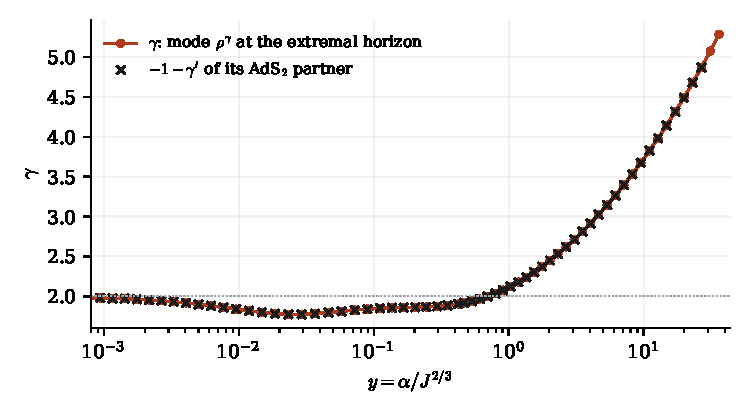
\includegraphics[width=.72\textwidth]{../figures/fig3-exponent.pdf}
\caption{Exponent $\gamma$ of the growing perturbation $\delta\propto\rho^\gamma$
of the extremal throat, as a function of $y=\alpha/J^{2/3}$ (dots and line). The
crosses show $-1-\gamma'$ for the AdS$_2$ partner exponent $\gamma'$. They fall
on the same curve, which checks the pairing. Extremal Myers--Perry ($y=0$) has
$\gamma=2$ exactly.}
\label{fig:gamma}
\end{figure}

\paragraph{Why it matters.} A generic extremal solution contains this mode with
some non-zero amplitude, so near the horizon its metric functions behave like
$c_0+c_1\rho+c_\gamma\rho^\gamma+\dots$. For $\gamma<2$, which is the case for
$0<y<\Rgammacrosstwo$, they are once but not twice differentiable in $\rho$ at
the horizon. Two consequences follow:
\begin{itemize}
\item In KKR's coordinate $r$ one has $\rho\propto r^2$, so the solution contains
$r^{2\gamma}$. Their remark that the solutions take ``an approximate form as a
power series in $r$'' near the horizon is therefore an approximation, never an
exact statement at finite coupling.
\item Spectral methods converge exponentially for analytic functions but only
algebraically when such a term is present. Any quantity read from a high
derivative is affected most. Section~\ref{sec:method} shows how this decided the
choice of unknowns.
\end{itemize}
The phenomenon is the five-dimensional, Gauss--Bonnet counterpart of the result
of Horowitz, Kolanowski, Remmen and Santos \cite{HKRS2023}: higher-curvature
corrections make the horizons of asymptotically flat extremal rotating black
holes non-smooth. We have \emph{not} computed curvature components in a parallelly
propagated frame, so we make no claim about whether the horizon is singular in
their sense. Our statement is about the differentiability of the metric functions.

\section{The numerical method}
\label{sec:method}

\subsection{What makes the extremal problem hard}

A non-extremal horizon is a simple zero of $b$ and $f$, and the standard approach
of \cite{BKKR2010} (gauge $g=r^2$, horizon at $r=r_H$) handles it well. At an
extremal horizon $b$ and $f$ have a double zero. The obvious extension is to keep
$g=r^2$, factor $(r-r_H)^2$ out of $b$ and $f$, and solve for the smooth
remainders. \emph{This does not work.} We tried it with Chebyshev collocation, and
the linear systems became nearly singular as the resolution grew: condition
numbers reached $10^{12}$--$10^{13}$ and the smallest singular value tended to
zero. The reason is that in this gauge the nearby \emph{non-extremal} solutions
are also almost representable. Moving slightly off extremality multiplies both $b$
and $f$ by the same factor $\sim1/(x+\delta)$, which polynomials of high degree
can approximate ever better. The discrete problem cannot decide whether it is
extremal, and it becomes ill-conditioned. We abandoned this route.

\subsection{KKR's gauge and its two hidden zero modes}

KKR use a different gauge. With their parameter $a=1$ and $P_i=e^{2F_i}$,
\begin{equation}
\begin{gathered}
  b=\frac{P_1\,r^4}{u^2+1},\qquad f=\frac{r^2}{P_1\,u},\qquad g=P_2\,u,\qquad
  h=P_2P_3\,u\Bigl(1+\frac{1}{u^2}\Bigr),\\
  w=\frac{\sqrt2}{u^2+1}+W,\qquad u=r^2+1 ,
\end{gathered}
\label{eq:kkr}
\end{equation}
with four unknown functions $P_1,P_2,P_3,W$. At $P_i=1$, $W=0$ this is exactly
extremal Myers--Perry, with the degenerate horizon at $r=0$. The essential
feature is that the product
\begin{equation}
  b\,f=\frac{r^6}{u\,(u^2+1)}
\end{equation}
does not depend on the unknowns. A non-extremal solution would need $b$ and $f$
to have simple zeros at some $r_H>0$, which this product forbids. So the
representation excludes the neighbours that spoiled the previous attempt.

KKR's gauge alone did not give a well-posed problem either. We first solved it at
fixed $a$ and $\alpha$ and found that Newton's method converged to solutions
that differed from run to run, and that the Jacobian had null vectors. These null
vectors were smooth, the same at every resolution, and did not come from the
discretisation. We identified them as two \emph{exact} zero modes:
\begin{enumerate}
\item \textbf{Size.} The parameter $a$ is not the size of the black hole. At
fixed $a$ and $\alpha$ the horizon can still be rescaled, so there is a
one-parameter family of solutions. We remove it by fixing the size of the
horizon sphere, $g_H=P_2(0)=1$, which is the same unit $r_H=1$ the manuscript
uses.
\item \textbf{A leftover radial gauge.} The condition $bf=$ fixed does not fix
$r$ completely. The shift $r\to r+c\sqrt{bf}$ preserves it. This shift grows
like $r^3$ near the horizon and tends to a constant shift at infinity. We remove
it by demanding that $P_2$ have no $1/r$ term at infinity.
\end{enumerate}
We also learned something from a failed fix. Replacing one collocation equation
by the Hamiltonian constraint (the $f$-equation, which the gauge-fixed system
does not impose) made the conditioning \emph{worse}. The constraint is kept
only as a diagnostic.

\subsection{Coordinate, unknowns, and how the mass is read}

\paragraph{Radial coordinate.} We compactify KKR's $r$ as
$s=r/(1+r)\in[0,1]$, with the horizon at $s=0$ and infinity at $s=1$. We first
used $\xi=r^2/(1+r^2)$, which looks natural because the equations contain $r^2$.
But the leftover gauge mode $r^3$ becomes $\xi^{3/2}$, a non-smooth function, and
convergence was slow. In $s$, both $r^3$ and the $1/r^n$ tails at infinity are
smooth. The only non-smooth term left is the physical $r^{2\gamma}$ of
section~\ref{sec:nh}.

\paragraph{Unknowns.} Instead of $P_i$ themselves we solve for $Q_i$ defined by
\begin{equation}
  P_i=1+(1-s)^2\,Q_i\quad(i=1,2,3),\qquad W=(1-s)^2\,Q_4 .
  \label{eq:Q}
\end{equation}
Because $(1-s)^2\simeq1/r^2$ at large $r$, this builds three conditions into the
representation: asymptotic flatness, the absence of $1/r$ terms (which removes
the leftover gauge mode), and, most importantly, that the mass is a \emph{value}:
\begin{equation}
  P_1=1+\frac{2c_t}{r^2}+\dots,\qquad c_t=\tfrac12\,Q_1(s=1),\qquad
  M=\frac{3\pi}{4}\,(1-c_t).
  \label{eq:mass}
\end{equation}
In a first version we solved for $P_i$ directly. The mass then came from the
\emph{second derivative} $P_1''$ at $s=1$, which is sensitive to the slow,
algebraic decay of the Chebyshev coefficients caused by $r^{2\gamma}$ at the
other end of the domain. Figure~\ref{fig:conv} shows the effect. With $P$ as
unknowns the mass converges like $N^{-2}$ and is wrong by $10^{-5}$--$10^{-2}$ even
at $N=160$. With $Q$ it reaches the $10^{-7}$ level already at $N\approx48$.
The angular momentum is read from the conserved momentum \eqref{eq:J} in the
interior of the domain, which avoids the fourth derivative its asymptotic tail
would require. The horizon velocity is
$\Omega_H=\tfrac{1}{\sqrt2}+W(0)$.

\begin{figure}[t]
\centering
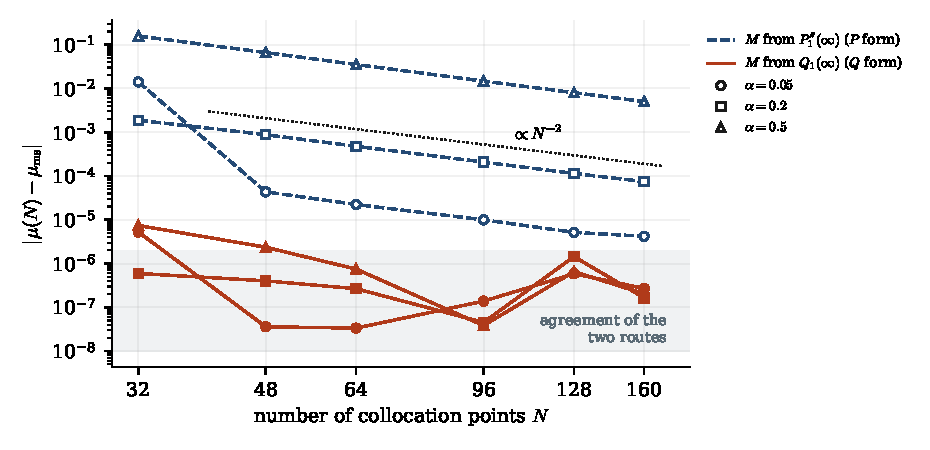
\includegraphics[width=.86\textwidth]{../figures/fig5-convergence.pdf}
\caption{Convergence of the extremal mass with the number of collocation points
$N$, at three couplings. The difference is taken from the manuscript's
independent $T\to0$ value $\mu_{\rm ms}$. Dashed: mass from the second derivative
of $P_1$ at infinity, which converges algebraically ($\propto N^{-2}$, fitted).
Solid: mass as the value $Q_1(\infty)$, eq.~\eqref{eq:mass}. The shaded band is
the level at which the two independent routes agree. Below it the comparison
cannot discriminate.}
\label{fig:conv}
\end{figure}

\subsection{Discretisation and solution}

The four equations for $(P_1,P_2,P_3,W)$ are the variations of the gauge-fixed
action. They are imposed at the $N$ Chebyshev--Gauss--Lobatto points of
$[0,1]$, with the following changes at the boundaries:
\begin{itemize}
\item At the horizon ($s=0$) the three $P$-equations are satisfied identically.
We replace them by $dP_i/ds=0$, which is the regularity condition (no odd power
$r^1$). The $W$-equation is kept.
\item At the first interior point the $W$-equation is replaced by the size
condition $P_2(0)=1$.
\item At infinity ($s=1$) all four equations are satisfied identically in the
$Q$ representation. They are imposed instead at a point midway between the last
two nodes.
\end{itemize}
The residuals are long rational expressions. They were generated symbolically
with SymPy and exported as NumPy code. To avoid catastrophic cancellation each is
written in three algebraically equivalent forms: expanded about the horizon for
$s\le0.12$, about infinity for $s\ge0.88$, and unexpanded in between. The
Jacobian is assembled analytically by the chain rule, with complex-step
derivatives of the residuals. It agrees with a brute-force complex-step Jacobian
of the whole discrete system to round-off. The nonlinear system is solved by
Newton's method with a backtracking line search.

\subsection{Following the branch}

At $\alpha=0$ the exact solution is $Q_i=0$ (extremal Myers--Perry). From there
we increase $\alpha$ step by step. Each solution is computed at two resolutions,
and a step is accepted only if all of the following hold:
\begin{itemize}
\item the residual is below $5\times10^{-8}$;
\item the Hamiltonian constraint, which is not imposed, is small;
\item the last Chebyshev coefficients of every function are below $10^{-5}$ of
the largest one, so the solution is resolved.
\end{itemize}
Each condition was added for a reason. The discrete system has \emph{spurious
roots}: solutions of the collocation equations whose Chebyshev coefficients do
not decay and that violate the constraint at the level of $10^{-3}$. Without the
constraint and tail tests Newton sometimes jumps onto one of them. Near the
round-off floor, Newton can also stop with grid-scale noise of order $10^{-6}$ in
the highest modes. When the tails show this we drop the top quarter of the
coefficients and solve again (a filtered restart). For $\alpha\gtrsim1$ the step
in $\alpha$ must be predicted along the tangent of the branch, $dQ/d\alpha$ (see
below), or Newton loses the physical root.

The branch was computed in four phases. The constraint threshold was relaxed and
the resolution raised as the solutions developed steeper structure near the
horizon:
\begin{itemize}
\item constraint $<10^{-6}$ and $N=48/72$ up to $\alpha\approx0.76$;
\item constraint $<10^{-5}$ and $N\ge96/144$ up to $\alpha\approx2.29$;
\item constraint $<10^{-4}$ and $N=128/192$ up to $\alpha\approx3.09$;
\item finally $N$ up to $\Rnmaxbranch$, ending at $\alpha=\Ralphamax$.
\end{itemize}
In total $\Rbranchpoints$ solutions were accepted. Going further was not possible
in double precision. The constraint violation, concentrated next to the horizon,
exceeded $10^{-4}$ even at $N=\Rnmaxbranch$. Raising $N$ does not help, because
the round-off floor of the residual grows with $N$. The best accuracy is reached
at $N\approx50$--$100$. One earlier attempt at $N=64/96$ was discarded because
round-off noise made the step size collapse.

\subsection{The slope without finite differences}

The slope $\partial M_\ext/\partial\alpha|_J$ could be obtained by differencing
masses at neighbouring couplings, but that divides the error by the step. Instead
we differentiate the discrete equations. If $R(Q;\alpha)=0$ is the collocation
system and $A=\partial R/\partial Q$ its Jacobian, then along the branch
\begin{equation}
  A\,\frac{dQ}{d\alpha}=-\frac{\partial R}{\partial\alpha},
  \label{eq:implicit}
\end{equation}
which costs one linear solve with the matrix Newton already has. From
$dQ/d\alpha$ we get $M_\alpha=dM/d\alpha=-\tfrac{3\pi}{8}\,dQ_1(1)/d\alpha$, and
$J_\alpha$ by a complex-step derivative of \eqref{eq:J}. Along our branch the
horizon size is fixed while $\alpha$ changes, so both $M$ and $J$ vary.
Differentiating $M=J^{2/3}\mu(y)$ with $y=\alpha J^{-2/3}$ gives
\begin{equation}
  \mu'(y)=\frac{M_\alpha-\tfrac23\,(M/J)\,J_\alpha}{1-\tfrac23\,(\alpha/J)\,J_\alpha}
  =\left.\frac{\partial M_\ext}{\partial\alpha}\right|_J .
  \label{eq:slope}
\end{equation}
The same tangent $dQ/d\alpha$ is the predictor used to follow the branch.

\section{Checks}
\label{sec:checks}

Every check listed here is evaluated in the code, and most are asserted (the
script stops if they fail).
\begin{enumerate}
\item \textbf{Myers--Perry limit.} At $\alpha=0$ the solver returns
$M=3\pi/4$, $J=\pi\sqrt2/4$, $\Omega_H=1/\sqrt2$, $S=2\pi J$, $j=1$ and
$a_H=s=\tfrac12$, the exact extremal Myers--Perry values.
\item \textbf{Constraint.} The Hamiltonian constraint is never imposed. Over the
whole branch it stays below $\Rconstraintworst$.
\item \textbf{Near-horizon data.} The horizon values of the full solutions must
coincide with the throat of section~\ref{sec:nh} at the same $\alpha/g_H$. With
$\rho\propto r^2$ the identification is $v_1=P_1(0)/4$ and $h_H=H_0$. They agree
to $\Rvonedev$ and $\RhHdev$ respectively.
\item \textbf{First law at $T=0$.} $\Psi=M_\alpha-2\Omega_HJ_\alpha$ along the
branch agrees with the slope \eqref{eq:slope} to $\Rfirstlawworst$ (median
$\Rfirstlawmedian$). This is over the $\Rcleanrows$ branch points where the two
resolutions agree to $10^{-5}$.
\item \textbf{Smarr at $T=0$.} $\Psi=(M-3\Omega_HJ)/\alpha$ agrees with the slope
to $\Rsmarrworst$ (median $\Rsmarrmedian$) for $\alpha\ge0.05$. At smaller
$\alpha$ the division by $\alpha$ amplifies errors.
\item \textbf{Scaling identity.} $3\Omega_HJ^{1/3}=\mu-y\mu'$ holds to
$\Romegaidclean$.
\item \textbf{Resolution.} Every quantity is computed at two (for the table, three)
resolutions, and the differences are reported. These are differences, not error
bounds.
\item \textbf{Independent re-run.} For this write-up the solver was run again from
scratch: from extremal Myers--Perry, in steps of $0.01$ up to $\alpha=0.2$ at
$N=64$. It reproduced the extremal Myers--Perry values to 12 digits. At the six
manuscript couplings in that range it matched the manuscript's $\mu$ to
$1\times10^{-7}$--$8\times10^{-7}$ and its $\Psi_\ext$ to better than
$2.2\times10^{-5}$ (receipt in appendix~\ref{app:repro}).
\end{enumerate}

\section{Results}
\label{sec:results}

\subsection{Profiles of the extremal solutions}

Figure~\ref{fig:profiles} shows the four functions of KKR's gauge,
$F_i=\tfrac12\ln P_i$ and $W$, for four couplings along the branch. All four
vanish identically for extremal Myers--Perry, so the curves show the deviation
caused by the Gauss--Bonnet term. The deviations are smooth and concentrated
within a few horizon radii ($s\lesssim0.7$, i.e.\ $r\lesssim2.3$). They grow
steadily with $\alpha$, and so do their gradients near the horizon, which is why
the resolution had to be raised along the branch. $F_2(0)=0$ is the size
condition $g_H=1$. The value $F_3(0)$ measures the squashing of the horizon
sphere, $h_H/g_H=2e^{2F_3(0)}$. It becomes more negative with coupling: the fibre
of the horizon, which for extremal Myers--Perry is elongated ($h_H/g_H=2$),
shrinks below the size of the round part ($h_H/g_H=1.21$, $0.74$, $0.56$ at
$\alpha=0.05$, $0.2$, $0.5$).

\begin{figure}[t]
\centering
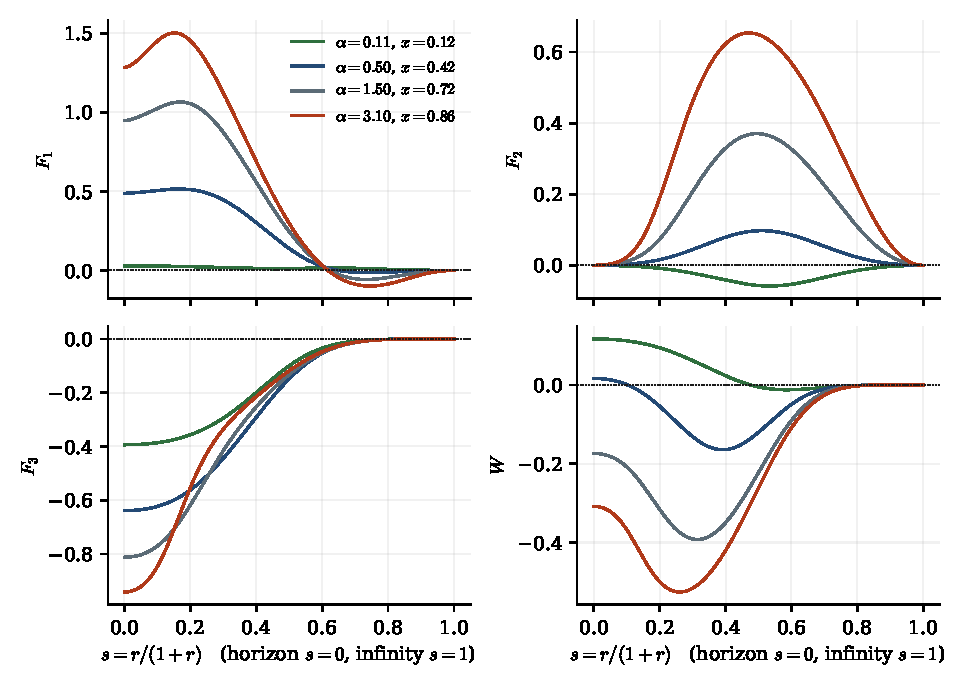
\includegraphics[width=.9\textwidth]{../figures/fig4-profiles.pdf}
\caption{The functions $F_i=\tfrac12\ln P_i$ and $W$ of eq.~\eqref{eq:kkr} for
extremal solutions at four couplings (units $g_H=1$), against the compactified
coordinate $s=r/(1+r)$. All vanish for extremal Myers--Perry.}
\label{fig:profiles}
\end{figure}

\subsection{Reproduction of KKR's domain of existence}

KKR plot the domain of existence of equal-spin black holes in the planes
$(x,a_H)$, $(x,s)$ and $(x,t_H)$, and against $j$ in insets. Its lower boundary
is the extremal set. To compare with our solutions we did not read the curves by
eye. The figures in the arXiv source are gnuplot EPS files, in which every curve
is a list of vertices in device coordinates. We extracted those vertices and
mapped them to data coordinates using each plot's own tick marks and labels.
The main plot and the inset were calibrated separately. Against the closed-form
static curves, which are also drawn in the figure, this calibration is accurate
to $\Rdigitworst$, about one device unit.

Figure~\ref{fig:fig1} shows the result. Our extremal branch (red) lies on KKR's
extremal curve (dashed blue) to $\RkkraHdev$ in $a_H(x)$ and $\Rkkrsdev$ in
$s(x)$. Against $j$ the agreement is $\RkkraHdevj$ and $\Rkkrsdevj$. These numbers
are at the level of the digitisation itself, so within what can be read from the
figure the curves coincide. KKR's bounds $j\le1$ and $x<1$ hold on the whole
branch, and $j$ falls to $\Rjlast$ at the end.

KKR continue to $x\approx0.92$. They draw a hand extrapolation from there to the
singular static configuration at $(x,j)=(1,0)$ and conjecture that the extremal
set ends there. Our branch ends at $x=\Rxmax$, for the numerical reasons given in
section~\ref{sec:method}, so we do not test that conjecture.

\begin{figure}[p]
\centering
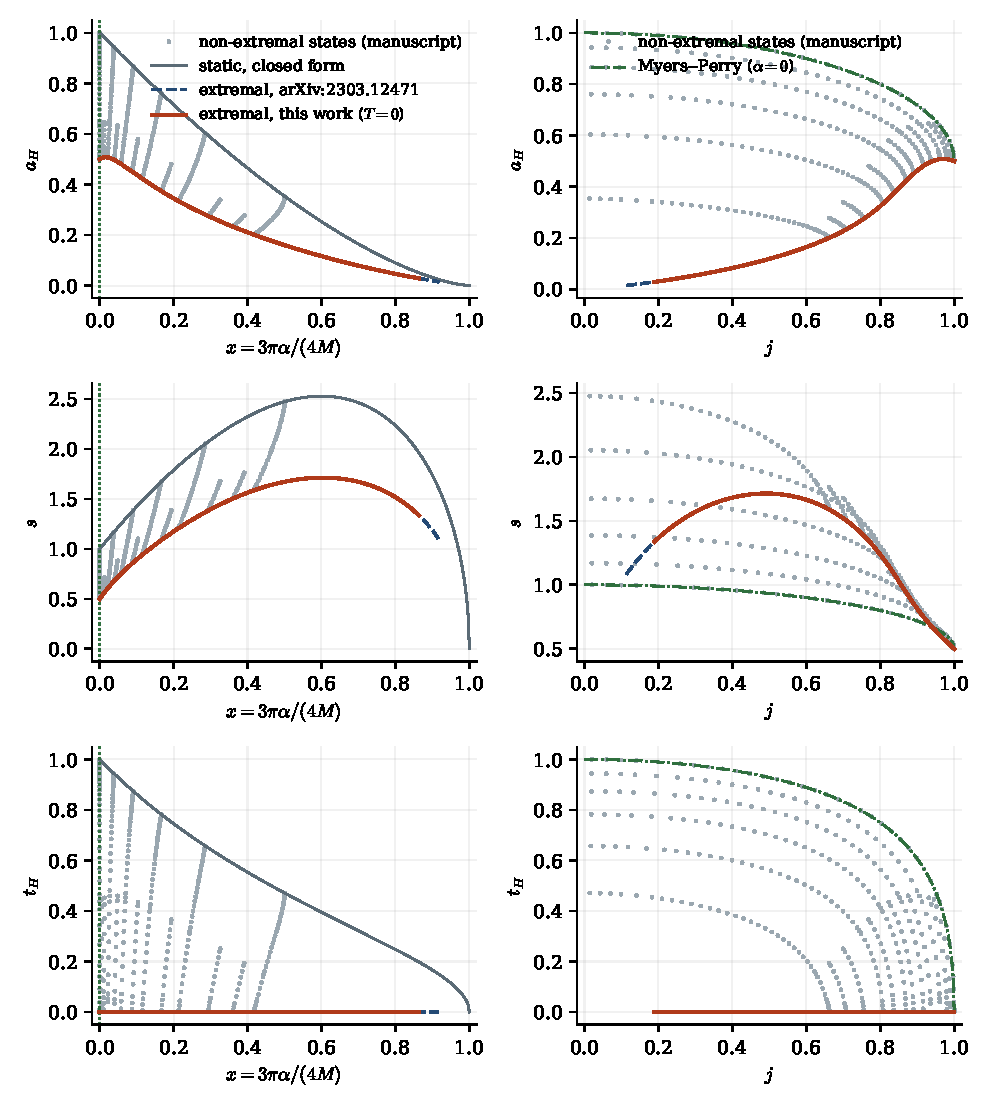
\includegraphics[width=\textwidth]{../figures/fig1-reproduction.pdf}
\caption{The equal-spin panels of figure~1 of KKR \cite{KKR2023}. Left: against
$x=3\pi\alpha/4M$. Right: against $j$ (their insets). Grey dots: non-extremal
black holes from the manuscript. Solid grey: the static family (closed form).
Dash-dotted green: Myers--Perry. Dashed blue: KKR's extremal curves, extracted
from their EPS files. Solid red: the extremal solutions constructed here at
$T=0$.}
\label{fig:fig1}
\end{figure}

\subsection{The extremal mass and its slope}

Figure~\ref{fig:shift} is the main physics result. The top panel shows the
extremal mass at fixed angular momentum, $\mu(y)=M_\ext/J^{2/3}$, together with
the first-order line $\mu(0)+\pi y$ of \eqref{eq:firstorder}. The middle panel
shows the slope $\mu'(y)=\partial M_\ext/\partial\alpha|_J$ from
\eqref{eq:slope}. The slope starts at the perturbative value $\pi$ and drops
quickly, to a minimum of $\Rslopemin$ at $y=\Rslopeminy$. It then rises slowly
again and reaches $\Rslopelast$ at the end of the branch ($y=\Rymax$). It never
changes sign. The extremal mass at fixed $J$ therefore increases with the
coupling throughout: the Gauss--Bonnet term tightens the extremality bound.
Over the branch $\mu$ grows by $\Rmugrowth\%$, well below the first-order line.

\begin{figure}[t]
\centering
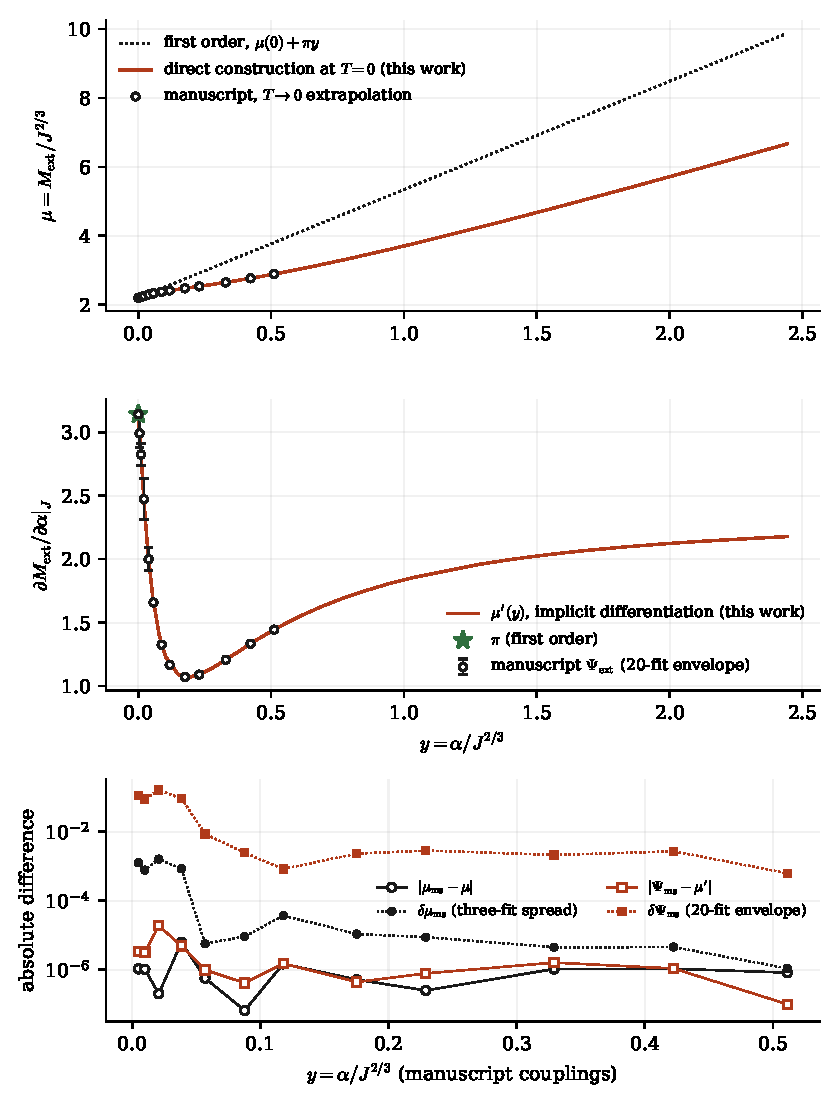
\includegraphics[width=.8\textwidth]{../figures/fig2-mass-shift.pdf}
\caption{Top: extremal mass at fixed angular momentum from the direct construction
(line), the manuscript's $T\to0$ extrapolations (circles), and the first-order
result (dotted). Middle: slope from implicit differentiation (line), its
first-order value $\pi$ (star), and the manuscript's $\Psi_\ext$ with its own
uncertainty envelope (error bars). Bottom: the differences between the two
routes (open symbols) compared with the manuscript's own uncertainty estimates
(filled symbols).}
\label{fig:shift}
\end{figure}

\paragraph{Comparison with the manuscript.} The manuscript obtains $\mu$ and the
slope $\Psi_\ext$ by fitting non-extremal solutions at low temperature and
extrapolating to $T=0$. It attaches two uncertainty estimates: the spread of
three fits of different degree for $\mu$, and a twenty-fit envelope for
$\Psi_\ext$. To compare at the same couplings we refined our solutions at each of
the manuscript's $\Rpolishedcouplings$ finite couplings with $N=64$, $96$ and
$128$ (table~\ref{tab:compare}). Across all of them:
\begin{itemize}
\item $y$ agrees to $\Rdyworstms$;
\item $\mu$ agrees to $\Rdmuworstms$;
\item the slope agrees to $\Rdpsiworstms$, which is at most $\Rpsiratioworst$ of
the manuscript's own envelope.
\end{itemize}
The two routes share no numerical machinery: different gauges, different
discretisations, and an extrapolation in temperature against none. They agree
far better than the manuscript's uncertainty estimates suggest. Those estimates
are therefore conservative. In a few cases the difference in $\mu$ exceeds the
manuscript's three-fit spread, but even then only at the level of $10^{-6}$.

\begin{table}[t]
\centering\footnotesize
\setlength{\tabcolsep}{2.6pt}
\begin{tabular}{@{}cccccccccc@{}}
\toprule
$\alpha$ & $y$ & $\mu$ (here) & res. & $\mu$ (ms) & spread &
$\mu'$ (here) & res. & $\Psi_\ext$ (ms) & envelope\\
\midrule
\Rcomparisontable
\bottomrule
\end{tabular}
\caption{Extremal solutions constructed at $T=0$ (here) against the manuscript's
$T\to0$ extrapolation (ms), at the manuscript's couplings ($g_H=1$). ``res.'' is
the larger of the differences between $N=128$ and $96$ and between $96$ and $64$.
``spread'' is the manuscript's three-fit spread of $\mu$ and ``envelope'' its
twenty-fit envelope for $\Psi_\ext$.}
\label{tab:compare}
\end{table}

\paragraph{Evidence for the non-smooth horizon in the full solutions.} The
exponent $\gamma$ comes from the linear analysis of section~\ref{sec:nh}. The full
solutions are consistent with it in three ways. The mass read from a second
derivative converges only algebraically (figure~\ref{fig:conv}), while an
analytic solution would converge exponentially. The constraint violation peaks
next to the horizon. So do the differences between resolutions. A direct fit of
the decay of the Chebyshev coefficients does \emph{not} resolve $\gamma$, however.
The coefficients reach the round-off plateau by mode $n\approx\Rgcplateau$, before
the algebraic decay $n^{-(4\gamma+1)}$ becomes visible. The full solutions
support the non-smooth horizon but do not measure its exponent independently.

\section{What was not established}
\label{sec:limits}

\begin{itemize}
\item \textbf{The endpoint.} Our branch stops at $x=\Rxmax$ ($\alpha=\Ralphamax$,
$y=\Rymax$). KKR reach $x\approx0.92$. Their conjecture that the extremal set ends
at the singular static point $(x,j)=(1,0)$ is not tested. Extending the branch
would need a coordinate that stretches the region next to the horizon, or
extended-precision arithmetic, not more continuation steps.
\item \textbf{Error bounds.} The resolution differences quoted throughout are
differences, not bounds. The round-off floor grows with $N$ and limits $\mu$ to
about $10^{-7}$--$10^{-6}$.
\item \textbf{Horizon regularity.} The non-integer exponent is established by the
linear analysis only. We did not compute curvature in a parallelly propagated
frame, so we do not claim a curvature singularity.
\item \textbf{Field equations.} They were checked against the tensor equations on
generic functions and against the closed-form static and Myers--Perry solutions.
The near-horizon identification is KKR's and was used as given.
\item \textbf{KKR's figure.} We compare with KKR's curves only on the range we
construct and make no statement about their accuracy beyond the figure. KKR's
scan of the interior of the domain of existence was not repeated. The interior
points in figure~\ref{fig:fig1} are the manuscript's ($\alpha\le\tfrac12$).
\item \textbf{Recalled, not derived.} The interpretation of the exponent pairing
as an AdS$_2$ property, and the relation to \cite{HKRS2023}, are recalled from the
literature (the abstract of \cite{HKRS2023} was re-read for this write-up). The
identities \eqref{eq:identities} and the slope formula \eqref{eq:slope} were
derived here.
\end{itemize}

\section{Summary}

The extremal equal-spin black holes of five-dimensional Einstein--Gauss--Bonnet
gravity can be built directly at zero temperature in KKR's gauge. Doing so
reliably needed three things beyond what KKR describe:
\begin{itemize}
\item removing two exact zero modes of the gauge (the size, and a leftover
radial reparametrisation);
\item a compactified coordinate in which the leftover gauge mode is smooth;
\item unknowns in which the mass is a value at infinity rather than a
derivative.
\end{itemize}
The last point matters because the extremal horizon carries a non-integer power
$\rho^\gamma$ at finite coupling, which slows the convergence of anything read
from high derivatives.

With these solutions we reproduce KKR's extremal curves to the precision of their
figure. We also obtain the extremal mass and its slope at fixed angular momentum
with no extrapolation in temperature. The slope falls from $\pi$ to $\Rslopemin$
and rises again, but stays positive, so the extremality bound tightens with the
coupling. Both the mass and the slope agree with the manuscript's extrapolated
values to a few parts in $10^6$: an independent confirmation of the
manuscript's central numbers, and evidence that its quoted uncertainties are
conservative.

\appendix
\section{Reproducing the results}
\label{app:repro}

All files are in \texttt{work/kkr-extremal}. Use the project environment
(\texttt{.venv}: Python 3.10.12, NumPy 2.2.6, SciPy 1.15.3, SymPy 1.14.0). In
order:
\begin{center}\small
\begin{tabular}{@{}p{.47\textwidth}p{.49\textwidth}@{}}
\toprule
command & produces \\
\midrule
\texttt{python derive.py} & field equations with $g$ free, checked against the tensor route \\
\texttt{python nearhorizon.py} & throat, KKR closed forms, exponents $\gamma(y)$ \\
\texttt{python kkr\_equations.py 0} & residuals in KKR's gauge as NumPy code ($\sim$7 min) \\
\texttt{python pw\_generator.py 0} & angular momentum from the conserved momentum \\
\texttt{python test\_rq.py} & solver gate and resolution study \\
\texttt{python branch\_rq.py \dots} & the extremal branch (several phases, resumable) \\
\texttt{python polish\_couplings.py} & high-resolution solutions at the manuscript's couplings \\
\texttt{python eps\_digitise.py}; \texttt{python kkr\_curves.py} & KKR's curves from their EPS files \\
\texttt{python analyse\_branch.py} & checks and comparisons \\
\texttt{python -m marimo export html figures\_kkr.py -o figures\_kkr.html} & figures \\
\texttt{python make\_report\_numbers.py} & every number quoted in this report \\
\bottomrule
\end{tabular}
\end{center}
The arXiv source of \cite{KKR2023} (needed for the EPS files) is not
redistributed. It is fetched from \texttt{https://arxiv.org/e-print/2303.12471}
into \texttt{arxiv/}. The original computation ran on 7 October 2026: the branch
from 09:47 to 14:10, and the refined solutions from 10:29 to 10:46.
\texttt{RESUME.txt} records the resume commands and the dead ends in more detail.

\paragraph{Receipt for this write-up (2026-10-07, 16:03--16:07).} The figure
notebook was re-run (\texttt{python -m marimo export html figures\_kkr.py}), which
added figures~\ref{fig:profiles} and~\ref{fig:conv}. The solver was re-run from
scratch as a spot check (extremal Myers--Perry start, $\alpha$ in steps of 0.01
to 0.2, $N=64$, 245\,s). Output:
{\footnotesize
\begin{verbatim}
alpha=0: M=2.356194490192 (3pi/4=2.356194490192)  J=1.110720734540
         (pi sqrt2/4=1.110720734540)  Omega_H=0.707106781187
alpha=0.010 mu=2.22627827 ms=2.22627878 d=5.1e-07 | mu'=2.8245634 Psi_ms=2.8245576
alpha=0.020 mu=2.25505852 ms=2.25505786 d=6.6e-07 | mu'=2.4728489 Psi_ms=2.4728269
alpha=0.050 mu=2.32801712 ms=2.32801721 d=9.7e-08 | mu'=1.6590803 Psi_ms=1.6590800
alpha=0.100 mu=2.41072791 ms=2.41072869 d=7.8e-07 | mu'=1.1662206 Psi_ms=1.1662137
alpha=0.150 mu=2.47399296 ms=2.47399319 d=2.3e-07 | mu'=1.0714928 Psi_ms=1.0714924
alpha=0.200 mu=2.53193599 ms=2.53193626 d=2.7e-07 | mu'=1.0900711 Psi_ms=1.0900703
\end{verbatim}}
The branch, the refined solutions and the near-horizon scan were not re-run for
this write-up. Their numbers are taken from the stored outputs through
\texttt{../report/numbers.tex}.

\begin{thebibliography}{9}
\bibitem{KKR2023} B.~Kleihaus, J.~Kunz and E.~Radu, \emph{Phases of rotating black
objects in $d=5$ Einstein--Gauss--Bonnet theory}, arXiv:2303.12471.
\bibitem{BKKR2010} Y.~Brihaye, B.~Kleihaus, J.~Kunz and E.~Radu, \emph{Rotating
black holes with equal-magnitude angular momenta in $d=5$ Einstein--Gauss--Bonnet
theory}, arXiv:1010.0860.
\bibitem{MaLiLu2020} L.~Ma, Y.-Z.~Li and H.~L\"u, \emph{$D=5$ rotating black
holes in Einstein--Gauss--Bonnet gravity: mass and angular momentum in
extremality}, arXiv:2009.00015.
\bibitem{HKRS2023} G.~T.~Horowitz, M.~Kolanowski, G.~N.~Remmen and J.~E.~Santos,
\emph{Extremal Kerr black holes as amplifiers of new physics}, arXiv:2303.07358.
\bibitem{Sen2007} A.~Sen, \emph{Black hole entropy function, attractors and
precision counting of microstates}, arXiv:0708.1270.
\bibitem{JacobsonMyers1993} T.~Jacobson and R.~C.~Myers, \emph{Entropy of
Lovelock black holes}, arXiv:hep-th/9305016.
\bibitem{KastorRayTraschen2010} D.~Kastor, S.~Ray and J.~Traschen, \emph{Smarr
formula and an extended first law for Lovelock gravity}, arXiv:1005.5053.
\end{thebibliography}

\end{document}
